\chapter{Cahier des Charges Fonctionnel}

\section{Cahier des Charges Fonctionnel}
Les d\'eveloppeurs effectuent r\'eguli\`erement des calculs sur des flux de donn\'ees, ils ont besoins d'utilitaires simples et performants.
Notre but principal est d'offrir une alternative \`a la biblioth\`eque num-utils qui propose des utilitaires de calcul num\'erique. 
Cette biblioth\`eque est impl\'ement\'ee en Perl, l'adaptation en C devrait nous permettre d'obtenir de meilleures performances.
Voici le diagramme b\^ete \`a corne qui pr\'esente de fa\c con tr\`es g\'en\'erale le programme que nous devons livrer : 

\begin{figure}[h]
\begin{center}
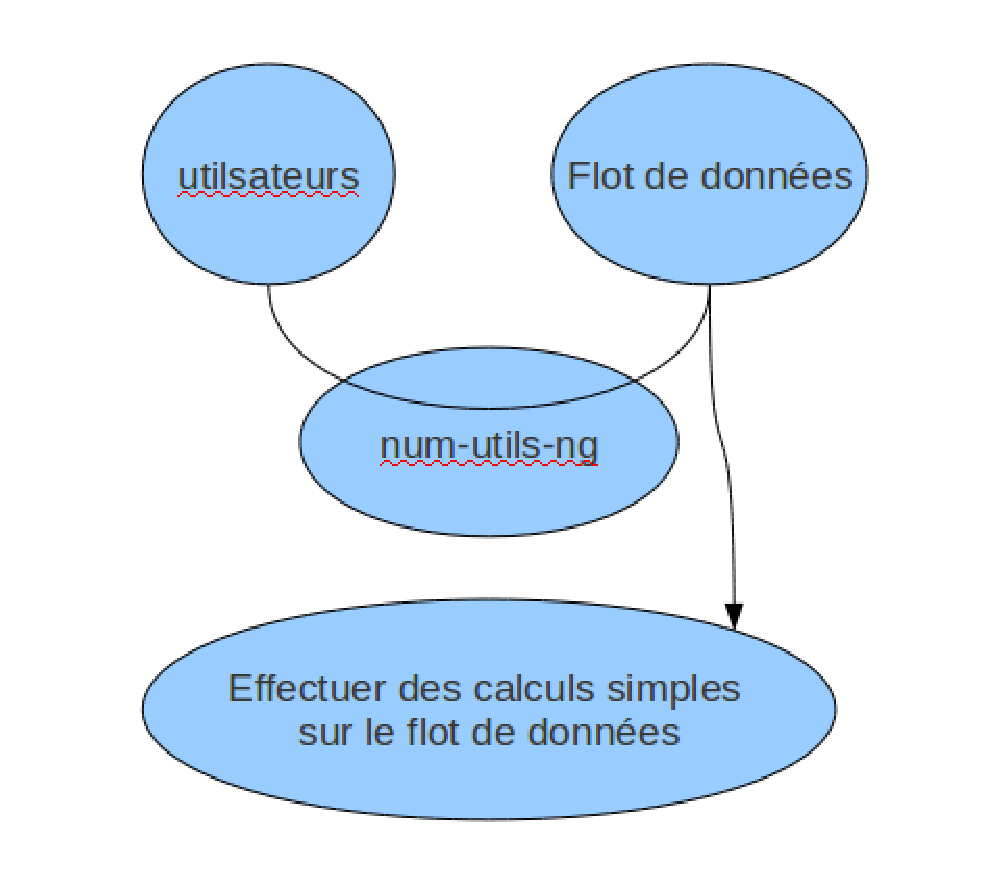
\includegraphics[width=9cm]{beteacorne.eps}
\end{center}
\caption{Diagramme B\^ete \`a cornes}
\label{fig:numprocess}
\end{figure}

Nous avons distingu\'e plusieurs fonctions contraintes pour notre biblioth\`eque : 
\newline
FP1 : Pouvoir effectuer des calculs simples sur des flots de donn\'ees.
\newline
FC3 : Cette biblioth\`eque doit \^etre \'ecrite dans un certain langage.
\newline
FC1 : Les utilitaires propos\'es doivent \^etre plus rapide que les anciens.
\newline
FC6 : La biblioth\`eque finale devra \^etre accessible  \`a tous.
\newline
FC4 : Les programmes doivent \^etre libre.
\newline
FC2 : La biblioth\`eque doit \^etre pr\^ete sous un certain d\'elai.
\newline
FC5 : Les utilisateurs doivent pouvoir se servir facilement de ces utilitaires.
\newline
FC7 : Il ne doit pas y avoir de bogues.
\newline


Les fonctions contraintes sont expos\'ees plus pr\'ecis\'ement dans le tableau fonctionnel ci-dessous.

\begin{table}[h]
\begin{center}
\begin{tabular}{|c|c|c|c|}
\hline
 & Crit\`ere & Niveau & Flexibilit\'e \\
\hline
 FC1 & Rapidit\'e & 10 fois plus rapide & 2 \\
\hline
 FC2 & D\'elai & 5 mois & 0 \\
\hline
 FC3 & Langage & C & 1 \\
\hline
 FC4 & Licence & GNU General Public License & 0 \\
\hline
 FC5 & Facilit\'e d'utilisation & M\^eme commandes qu'avant & 2 \\
\hline
 FC6 & Accessibilit\'e & Disponible sur le d\'ep\^ot officiel Debian & 1 \\
\hline
 FC7 & Nombre de bogues & 0 & 1 \\
\hline
\end{tabular}
\caption{Tableau Fonctionnel}
\end{center}
\label{tab:tabfonctionnel}
\end{table}

Flexibilit\'e : \newline
0 = imp\'eratif\newline
1 = peu n\'egociable\newline
2 = n\'egociable\newline
3 = tr\`es n\'egociable\newline



